% =============================================================================
%  The assumptions of a one-dimensional PBL closure -- GRAPH version (prototype, A3 landscape)
%  GENERATED by scripts/make_pyramid_graph.py from pbl_assumptions_pyramid.tex. Tiers as rows, titles
%  only; contacts derived from the block geometry (thick, bundled into the parent), leans from the
%  \lean entries (thin arrows; dashed within a tier). Edit the horizontal file and regenerate.
% =============================================================================
\documentclass[10pt]{article}
\usepackage{iftex}
\ifPDFTeX
  \usepackage[utf8]{inputenc}
  \usepackage[T1]{fontenc}
  \usepackage{lmodern}
\else
  \usepackage{fontspec}
  \setmainfont{lmroman10-regular.otf}[BoldFont=lmroman10-bold.otf,
    ItalicFont=lmroman10-italic.otf, BoldItalicFont=lmroman10-bolditalic.otf]
\fi
\usepackage[british]{babel}
\usepackage[paperwidth=42cm,paperheight=29.7cm,margin=12mm]{geometry}
\usepackage{amsmath,amssymb}
\usepackage{xcolor}
\usepackage{tikz}
\usetikzlibrary{arrows.meta,calc}
\usepackage{microtype}
\pagestyle{empty}
\setlength{\parindent}{0pt}
\setlength{\parskip}{0.5ex}
% rigid math relation spacing: the centred block texts would otherwise stretch around = and <<
\thickmuskip=5mu \medmuskip=4mu \thinmuskip=3mu

% ---- notation ---------------------------------------------------------------
\newcommand{\avg}[1]{\langle #1 \rangle}
\newcommand{\pd}[2]{\partial #1/\partial #2}
\newcommand{\qsq}{q^{2}}
\newcommand{\Rfc}{R_{fc}}
\newcommand{\dx}{\Delta x}
% ---- rows the PhD concept turns on (same data as the note's macros.tex) ------
\definecolor{cKey}{HTML}{7B2D8E}
\definecolor{cGXIX}{HTML}{990011}   % Goger 2019 port (the note's colour)
\definecolor{cFULL}{HTML}{7B2D8E}   % Kosovic-Juliano 3D closure (the note's colour)
% \hl{x0}{x1}{y0}{y1}{colour}{inset}: a frame inside a block, marking a scheme's decisive block
\newcommand{\hl}[6]{\draw[#5, line width=1.1pt] (#1+#6,#3+#6) rectangle (#2-#6,#4-#6);}
\newcommand{\setkey}[2]{\expandafter\def\csname key@#1\endcsname{#2}}
\makeatletter
\setkey{A1}{1}\setkey{B1}{1}\setkey{B2}{1}\setkey{B3}{1}\setkey{C3}{1}\setkey{C4}{1}\setkey{C6}{1}\setkey{C7}{1}
\setkey{B5}{2}\setkey{B6}{2}\setkey{C2}{2}\setkey{C5}{2}\setkey{C9}{2}
\newcommand{\keymark}[1]{\ifcsname key@#1\endcsname
  \if1\csname key@#1\endcsname\textcolor{cKey}{$\blacktriangleright$}\else\textcolor{cKey}{$\triangleright$}\fi\fi}
\makeatother
\newcommand{\pid}[1]{\keymark{#1}\textbf{#1}}
% \pb{x0}{x1}{y0}{y1}{style}{text}: a block from (x0,y0) to (x1,y1), text centred
\newcommand{\pbf}[7]{\pgfmathsetmacro{\pbw}{#2-#1-#7}%
  \draw[#5] (#1,#3) rectangle (#2,#4);
  \node[align=center, font=\tiny, inner sep=0pt, text width=\pbw cm] at ({(#1+#2)/2},{(#3+#4)/2}) {#6};}
\newcommand{\pb}[6]{\pgfmathsetmacro{\pbw}{#2-#1-0.20}%
  \draw[#5] (#1,#3) rectangle (#2,#4);
  \node[align=center, font=\tiny, inner sep=0pt, text width=\pbw cm] at ({(#1+#2)/2},{(#3+#4)/2}) {#6};}


% ---- the hectometre-scale column (used by the VERTICAL version only; read by scripts/make_pyramid_vertical.py)
% \hecto{<concept title>}{<what becomes of the concept at Delta = 500 m over the Inn Valley>}; no-op here.
% Sources: the mountain and grey-zone columns of the note's Table I.1 and the project's own runs.
\newcommand{\hecto}[2]{}
\hecto{Locality}{By day eddies span $z_i$ and the flux stops answering the local gradient; on slopes it arrives from the interface. Holds at night.}
\hecto{Reynolds averaging}{The cell mean is a filter of width $\Delta$ inside the spectrum: Leonard and cross terms appear; the closed term is a subfilter stress.}
\hecto{Ergodicity in space}{At night a 500~m cell holds about five integral scales per direction and $\Delta z$ none: the cell statistic is an order-one realisation. By day it holds less than one eddy. On a slope it mixes two flows, slope layer and valley core, and estimates neither.}
\hecto{Boundary-layer (column) approximation}{Not small: the cross-valley shear of the up-valley jet reaches 20--30\,\% of the vertical shear; slope flows carry $W$ gradients of the order of the wind shear; horizontal flux divergences are of the order of the vertical one, and the Riviera budgets closed only with transport and advection. Seven of nine production terms and the three-dimensional divergences are missing, not negligible.}
\hecto{Constant-flux layer}{The katabatic jet nose at 2--10~m sits inside the layer; the momentum flux is height-constant in 8--28\,\% of daytime periods.}
\hecto{Local equilibrium}{Resolved strain by day rotates faster than $l/q$; transitions and intermittency at night are not slow against it.}
\hecto{Monin--Obukhov similarity}{A slope has two axes, gravity and the surface normal: two Obukhov lengths, a slope-normal heat flux with a horizontal part. The scaling holds only for some anisotropy classes, and over a hill only in the inner layer. Over the forested slopes the first model level sits inside the roughness sublayer. At Innsbruck the surface is stable 4.7\,\% of the time while the valley air above is often stably stratified.}
\hecto{Mixing length}{$z_i$ ill-posed under elevated inversions, wall distance ambiguous on a slope; the valley width sets the horizontal eddy: two lengths.}
\hecto{Universal constants}{Fitted to flat neutral and convective layers; the anisotropy classes of complex terrain differ, and the comparison already runs three constant sets. Filter constants are not ensemble constants: $C_\varepsilon$ depends on $l/\Delta$.}
\hecto{Energy cascade}{$\varepsilon$ is filter-independent while $q^3$ is not: the dissipation length must shrink with the grid; by day the filter cuts into the isotropic range.}
\hecto{Return to isotropy}{Stable valley turbulence is two-component, pancake-like; the return rate of a pancake need not be that of a convective eddy. Pressure work by slope flows and gravity waves redistributes energy laterally, the least known term of the budget.}
\hecto{Eddy viscosity}{The grid filter, aspect ratio 25, imprints its anisotropy on the subgrid eddies; the stress axes turn where slope meets valley wind.}
\hecto{Buoyancy production}{The slope-normal surface heat flux has a horizontal component with no home in the budget; in stable air buoyancy damps $\avg{w^2}$ selectively, the pancake anisotropy; by day resolved thermals carry the horizontal heat flux and its subgrid part stays unrepresented.}



% ---- dependencies the contact rule cannot draw (post-audit list; used by scripts/make_pyramid_graph.py). No-op here.
\newcommand{\lean}[2]{}
\lean{Locality}{Mixing}
\lean{Boundary-layer (column) approximation}{Boussinesq}
\lean{Monin--Obukhov similarity}{Horizontal homogeneity}
\lean{Monin--Obukhov similarity}{Axisymmetry}
\lean{Mixing length}{Horizontal homogeneity}
\lean{Energy cascade}{Stationarity}
\lean{Local equilibrium}{Locality}
\lean{Eddy viscosity}{Locality}
\lean{Universal constants}{Reynolds averaging}
\lean{Vertical divergence only}{Scale separation}
\lean{Wall value of $\qsq$}{Universal constants}
\lean{Level-2.5 truncation}{Return to isotropy}
\lean{Level-2.5 truncation}{Universal constants}
\lean{Level-2.5 truncation}{Boundary-layer (column) approximation}
\lean{Master length scale}{Axisymmetry}
\lean{Pressure terms}{Locality}
\lean{Pressure terms}{Universal constants}
\lean{K-form fluxes}{Locality}
\lean{K-form fluxes}{Mixing length}
\lean{K-form fluxes}{Local equilibrium}
\lean{Dissipation}{Master length scale}
\lean{Resolved gradient}{Boundary-layer (column) approximation}
% ---- scheme quicklook (moons above the formalism tier; scripts/make_moons.py rewrites the strip)
% \moon{<block title>}{K|P|D x4} in the order MYNN as run, G19 port, 3D-APPROX, 3D-FULL; from Table I.0 of the note:
% a block is K if all its rows are kept, D if all are dropped, else P. No-op here (data only).
\newcommand{\moon}[2]{}
\moon{Resolved gradient}{K K K K}
\moon{Grid means are ensemble means}{P K P P}
\moon{Vertical shear only}{K P K D}
\moon{Vertical divergence only}{K P P D}
\moon{Wall value of $\qsq$}{K K D D}
\moon{Level-2.5 truncation}{P P K P}
\moon{Surface fluxes and first level}{K K K K}
\moon{Master length scale}{K P K K}
\moon{Constant set}{K K K K}
\moon{Dissipation}{K K K K}
\moon{Pressure terms}{K K K K}
\moon{K-form fluxes}{P P P D}
\moon{Buoyancy term}{P P P P}
% glyphs (the note's), absolute size, colour = scheme identity
\newcommand{\gK}{\tikz[baseline=-0.6ex]{\fill (0,0) circle (0.11);}}
\newcommand{\gP}{\tikz[baseline=-0.6ex]{\draw[line width=0.5pt] (0,0) circle (0.11); \fill (0,0) -- (90:0.11) arc (90:270:0.11) -- cycle;}}
\newcommand{\gD}{\tikz[baseline=-0.6ex]{\draw[line width=0.5pt] (0,0) circle (0.11);}}
\definecolor{cMYNN}{HTML}{3A6B00}    % MYNN as run
\definecolor{cAPPROX}{HTML}{9A5AA8}  % 3D-APPROX


\definecolor{cLean}{HTML}{1F5FA8}
\tikzset{nd/.style={draw, line width=0.4pt, align=center, font=\scriptsize, inner sep=3pt, minimum height=1.1cm},
  contact/.style={black!60, line width=1.2pt},
  lean/.style={cLean, line width=0.55pt, -{Stealth[length=4pt, width=3pt]}},
  leansame/.style={cLean, line width=0.55pt, dashed, -{Stealth[length=4pt, width=3pt]}},
  tier/.style={font=\small\bfseries, text=black!55, anchor=east}}
\begin{document}
{\Large\bfseries The assumptions of a one-dimensional PBL closure as a dependency graph}\\[0.3ex]
{\small Prototype of the graph view: the blocks of the pyramid as nodes, tiers as rows, every dependency drawn. 2026-09-16.}

\vspace{0.4ex}
{\footnotesize Thick grey lines are the pyramid's contacts, the primary parents, converging on the parent they enter.
Thin blue arrows are the further dependencies of the audit; dashed where both ends lie in one tier. Frames as on the
pyramid pages: \textcolor{cGXIX}{\textbf{red}} the Goger 2019 port, \textcolor{cFULL}{\textbf{purple}} the
Kosovi\'c--Juliano three-dimensional closure. Statements and the scheme quicklook are on the pyramid pages; this page
carries the structure only.\par}
\vspace{1ex}
\begin{center}
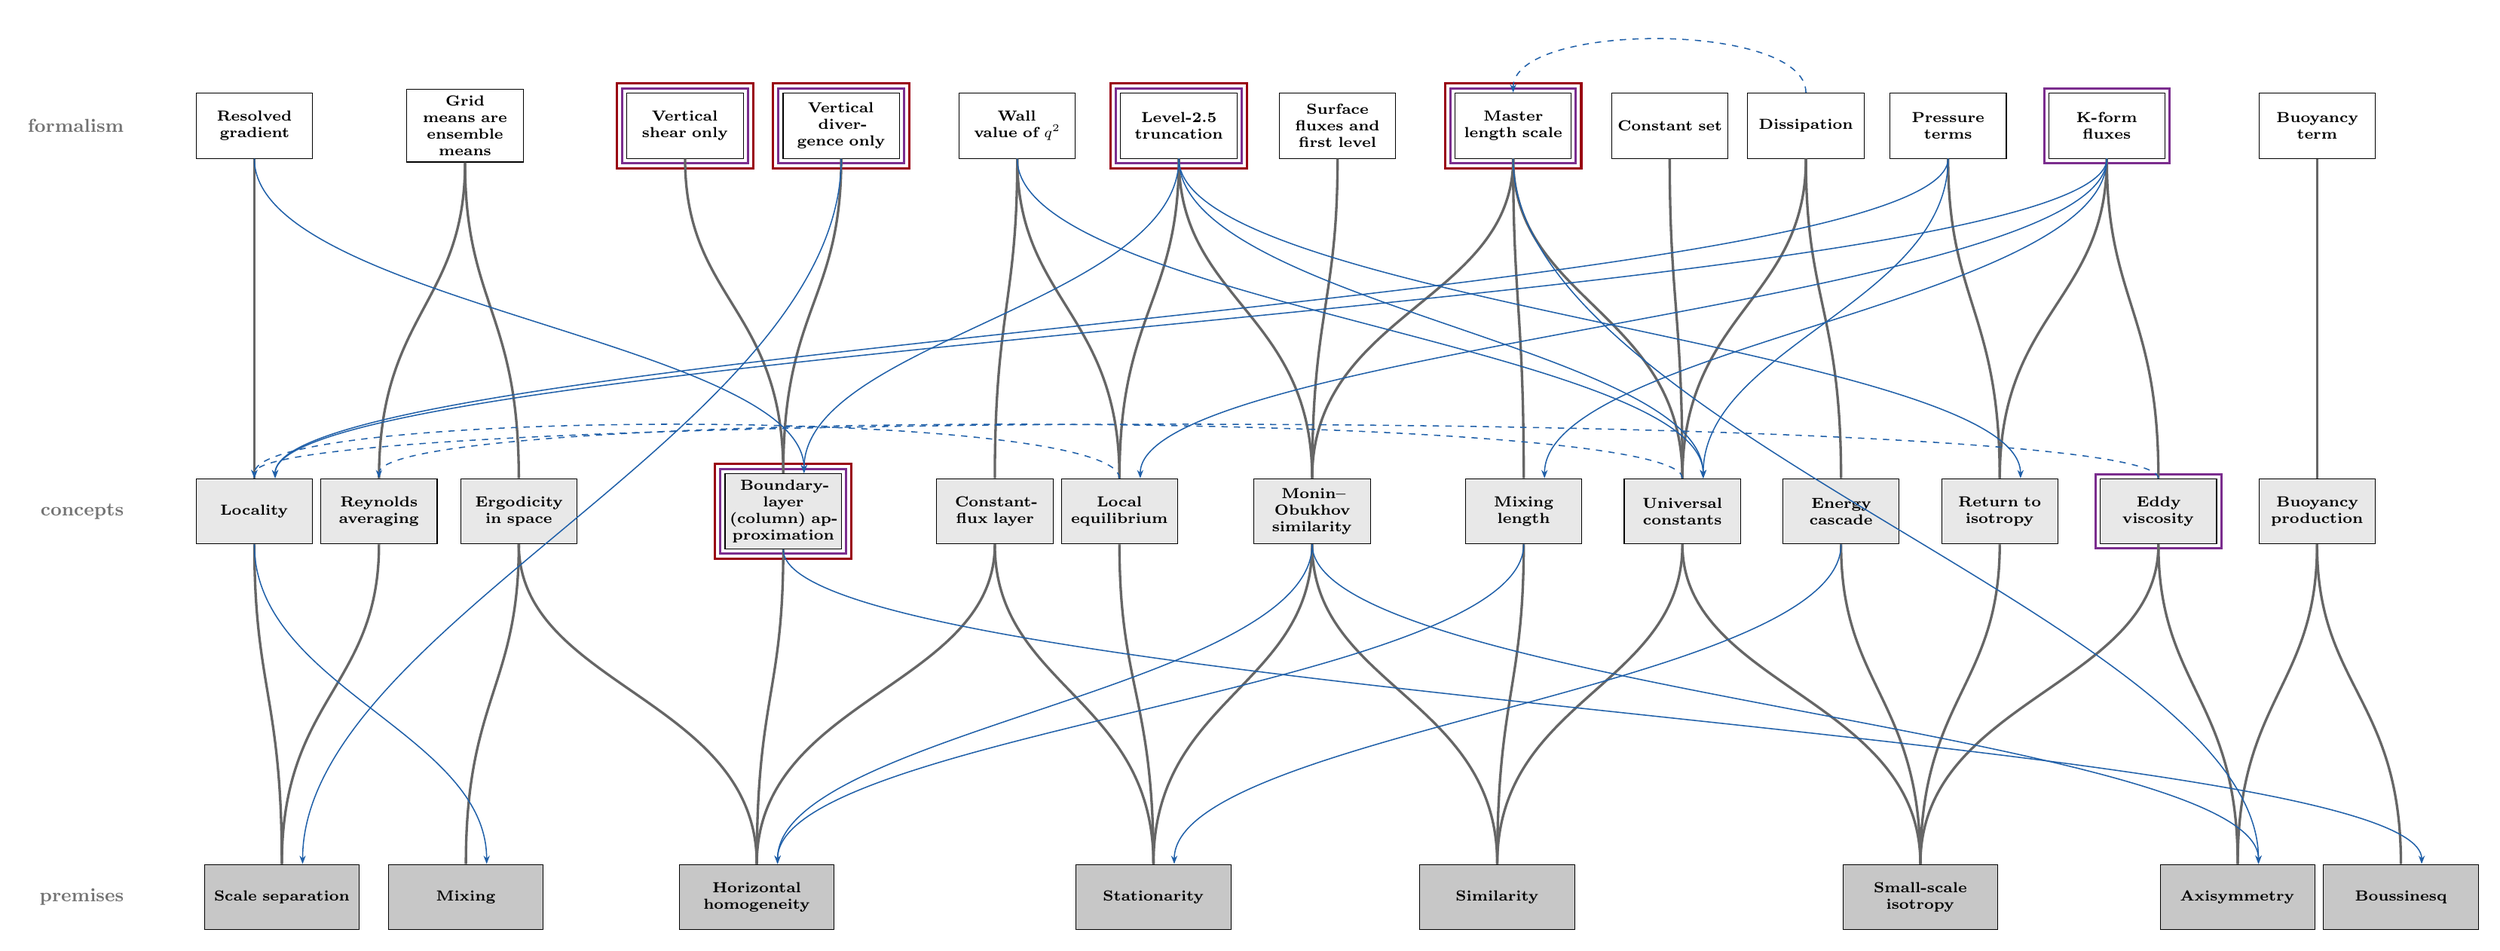
\begin{tikzpicture}[x=1cm, y=1cm]
\node[tier] at (-0.4, 13.0) {formalism};
\node[tier] at (-0.4, 6.5) {concepts};
\node[tier] at (-0.4, 0.0) {premises};
\node[nd, fill=black!22, text width=2.4cm] (n0) at (2.139,0.00) {\textbf{Scale separation}};
\node[nd, fill=black!22, text width=2.4cm] (n1) at (5.240,0.00) {\textbf{Mixing}};
\node[nd, fill=black!22, text width=2.4cm] (n2) at (10.142,0.00) {\textbf{Horizontal homogeneity}};
\node[nd, fill=black!22, text width=2.4cm] (n3) at (16.826,0.00) {\textbf{Stationarity}};
\node[nd, fill=black!22, text width=2.4cm] (n4) at (22.619,0.00) {\textbf{Similarity}};
\node[nd, fill=black!22, text width=2.4cm] (n5) at (29.749,0.00) {\textbf{Small-scale isotropy}};
\node[nd, fill=black!22, text width=2.4cm] (n6) at (35.096,0.00) {\textbf{Axisymmetry}};
\node[nd, fill=black!22, text width=2.4cm] (n7) at (37.846,0.00) {\textbf{Boussinesq}};
\node[nd, fill=black!9, text width=1.75cm] (n8) at (1.676,6.50) {\textbf{Locality}};
\node[nd, fill=black!9, text width=1.75cm] (n9) at (3.776,6.50) {\textbf{Reynolds averaging}};
\node[nd, fill=black!9, text width=1.75cm] (n10) at (6.132,6.50) {\textbf{Ergodicity in space}};
\node[nd, fill=black!9, text width=1.75cm] (n11) at (10.588,6.50) {\textbf{Boundary-layer (column) approximation}};
\node[nd, fill=black!9, text width=1.75cm] (n12) at (14.153,6.50) {\textbf{Constant-flux layer}};
\node[nd, fill=black!9, text width=1.75cm] (n13) at (16.253,6.50) {\textbf{Local equilibrium}};
\node[nd, fill=black!9, text width=1.75cm] (n14) at (19.500,6.50) {\textbf{Monin--Obukhov similarity}};
\node[nd, fill=black!9, text width=1.75cm] (n15) at (23.065,6.50) {\textbf{Mixing length}};
\node[nd, fill=black!9, text width=1.75cm] (n16) at (25.739,6.50) {\textbf{Universal constants}};
\node[nd, fill=black!9, text width=1.75cm] (n17) at (28.412,6.50) {\textbf{Energy cascade}};
\node[nd, fill=black!9, text width=1.75cm] (n18) at (31.086,6.50) {\textbf{Return to isotropy}};
\node[nd, fill=black!9, text width=1.75cm] (n19) at (33.760,6.50) {\textbf{Eddy viscosity}};
\node[nd, fill=black!9, text width=1.75cm] (n20) at (36.433,6.50) {\textbf{Buoyancy production}};
\node[nd, fill=white, text width=1.75cm] (n21) at (1.676,13.00) {\textbf{Resolved gradient}};
\node[nd, fill=white, text width=1.75cm] (n22) at (5.226,13.00) {\textbf{Grid means are ensemble means}};
\node[nd, fill=white, text width=1.75cm] (n23) at (8.934,13.00) {\textbf{Vertical shear only}};
\node[nd, fill=white, text width=1.75cm] (n24) at (11.565,13.00) {\textbf{Vertical divergence only}};
\node[nd, fill=white, text width=1.75cm] (n25) at (14.531,13.00) {\textbf{Wall value of $\qsq$}};
\node[nd, fill=white, text width=1.75cm] (n26) at (17.254,13.00) {\textbf{Level-2.5 truncation}};
\node[nd, fill=white, text width=1.75cm] (n27) at (19.928,13.00) {\textbf{Surface fluxes and first level}};
\node[nd, fill=white, text width=1.75cm] (n28) at (22.887,13.00) {\textbf{Master length scale}};
\node[nd, fill=white, text width=1.75cm] (n29) at (25.525,13.00) {\textbf{Constant set}};
\node[nd, fill=white, text width=1.75cm] (n30) at (27.820,13.00) {\textbf{Dissipation}};
\node[nd, fill=white, text width=1.75cm] (n31) at (30.216,13.00) {\textbf{Pressure terms}};
\node[nd, fill=white, text width=1.75cm] (n32) at (32.890,13.00) {\textbf{K-form fluxes}};
\node[nd, fill=white, text width=1.75cm] (n33) at (36.433,13.00) {\textbf{Buoyancy term}};
\draw[cFULL, line width=1.1pt] ($(n11.south west)+(-0.07,-0.07)$) rectangle ($(n11.north east)+(0.07,0.07)$);
\draw[cGXIX, line width=1.1pt] ($(n11.south west)+(-0.16,-0.16)$) rectangle ($(n11.north east)+(0.16,0.16)$);
\draw[cFULL, line width=1.1pt] ($(n23.south west)+(-0.07,-0.07)$) rectangle ($(n23.north east)+(0.07,0.07)$);
\draw[cGXIX, line width=1.1pt] ($(n23.south west)+(-0.16,-0.16)$) rectangle ($(n23.north east)+(0.16,0.16)$);
\draw[cFULL, line width=1.1pt] ($(n24.south west)+(-0.07,-0.07)$) rectangle ($(n24.north east)+(0.07,0.07)$);
\draw[cGXIX, line width=1.1pt] ($(n24.south west)+(-0.16,-0.16)$) rectangle ($(n24.north east)+(0.16,0.16)$);
\draw[cFULL, line width=1.1pt] ($(n26.south west)+(-0.07,-0.07)$) rectangle ($(n26.north east)+(0.07,0.07)$);
\draw[cGXIX, line width=1.1pt] ($(n26.south west)+(-0.16,-0.16)$) rectangle ($(n26.north east)+(0.16,0.16)$);
\draw[cFULL, line width=1.1pt] ($(n28.south west)+(-0.07,-0.07)$) rectangle ($(n28.north east)+(0.07,0.07)$);
\draw[cGXIX, line width=1.1pt] ($(n28.south west)+(-0.16,-0.16)$) rectangle ($(n28.north east)+(0.16,0.16)$);
\draw[cFULL, line width=1.1pt] ($(n19.south west)+(-0.07,-0.07)$) rectangle ($(n19.north east)+(0.07,0.07)$);
\draw[cFULL, line width=1.1pt] ($(n32.south west)+(-0.07,-0.07)$) rectangle ($(n32.north east)+(0.07,0.07)$);
\draw[contact] (n8.south) .. controls ($(n8.south)+(0,-2.4)$) and ($(n0.north)+(0,2.8)$) .. (n0.north);
\draw[contact] (n9.south) .. controls ($(n9.south)+(0,-2.4)$) and ($(n0.north)+(0,2.8)$) .. (n0.north);
\draw[contact] (n10.south) .. controls ($(n10.south)+(0,-2.4)$) and ($(n1.north)+(0,2.8)$) .. (n1.north);
\draw[contact] (n10.south) .. controls ($(n10.south)+(0,-2.4)$) and ($(n2.north)+(0,2.8)$) .. (n2.north);
\draw[contact] (n11.south) .. controls ($(n11.south)+(0,-2.4)$) and ($(n2.north)+(0,2.8)$) .. (n2.north);
\draw[contact] (n12.south) .. controls ($(n12.south)+(0,-2.4)$) and ($(n2.north)+(0,2.8)$) .. (n2.north);
\draw[contact] (n12.south) .. controls ($(n12.south)+(0,-2.4)$) and ($(n3.north)+(0,2.8)$) .. (n3.north);
\draw[contact] (n13.south) .. controls ($(n13.south)+(0,-2.4)$) and ($(n3.north)+(0,2.8)$) .. (n3.north);
\draw[contact] (n14.south) .. controls ($(n14.south)+(0,-2.4)$) and ($(n3.north)+(0,2.8)$) .. (n3.north);
\draw[contact] (n14.south) .. controls ($(n14.south)+(0,-2.4)$) and ($(n4.north)+(0,2.8)$) .. (n4.north);
\draw[contact] (n15.south) .. controls ($(n15.south)+(0,-2.4)$) and ($(n4.north)+(0,2.8)$) .. (n4.north);
\draw[contact] (n16.south) .. controls ($(n16.south)+(0,-2.4)$) and ($(n4.north)+(0,2.8)$) .. (n4.north);
\draw[contact] (n16.south) .. controls ($(n16.south)+(0,-2.4)$) and ($(n5.north)+(0,2.8)$) .. (n5.north);
\draw[contact] (n17.south) .. controls ($(n17.south)+(0,-2.4)$) and ($(n5.north)+(0,2.8)$) .. (n5.north);
\draw[contact] (n18.south) .. controls ($(n18.south)+(0,-2.4)$) and ($(n5.north)+(0,2.8)$) .. (n5.north);
\draw[contact] (n19.south) .. controls ($(n19.south)+(0,-2.4)$) and ($(n5.north)+(0,2.8)$) .. (n5.north);
\draw[contact] (n19.south) .. controls ($(n19.south)+(0,-2.4)$) and ($(n6.north)+(0,2.8)$) .. (n6.north);
\draw[contact] (n20.south) .. controls ($(n20.south)+(0,-2.4)$) and ($(n6.north)+(0,2.8)$) .. (n6.north);
\draw[contact] (n20.south) .. controls ($(n20.south)+(0,-2.4)$) and ($(n7.north)+(0,2.8)$) .. (n7.north);
\draw[contact] (n21.south) .. controls ($(n21.south)+(0,-2.4)$) and ($(n8.north)+(0,2.8)$) .. (n8.north);
\draw[contact] (n22.south) .. controls ($(n22.south)+(0,-2.4)$) and ($(n9.north)+(0,2.8)$) .. (n9.north);
\draw[contact] (n22.south) .. controls ($(n22.south)+(0,-2.4)$) and ($(n10.north)+(0,2.8)$) .. (n10.north);
\draw[contact] (n23.south) .. controls ($(n23.south)+(0,-2.4)$) and ($(n11.north)+(0,2.8)$) .. (n11.north);
\draw[contact] (n24.south) .. controls ($(n24.south)+(0,-2.4)$) and ($(n11.north)+(0,2.8)$) .. (n11.north);
\draw[contact] (n25.south) .. controls ($(n25.south)+(0,-2.4)$) and ($(n12.north)+(0,2.8)$) .. (n12.north);
\draw[contact] (n25.south) .. controls ($(n25.south)+(0,-2.4)$) and ($(n13.north)+(0,2.8)$) .. (n13.north);
\draw[contact] (n26.south) .. controls ($(n26.south)+(0,-2.4)$) and ($(n13.north)+(0,2.8)$) .. (n13.north);
\draw[contact] (n26.south) .. controls ($(n26.south)+(0,-2.4)$) and ($(n14.north)+(0,2.8)$) .. (n14.north);
\draw[contact] (n27.south) .. controls ($(n27.south)+(0,-2.4)$) and ($(n14.north)+(0,2.8)$) .. (n14.north);
\draw[contact] (n28.south) .. controls ($(n28.south)+(0,-2.4)$) and ($(n14.north)+(0,2.8)$) .. (n14.north);
\draw[contact] (n28.south) .. controls ($(n28.south)+(0,-2.4)$) and ($(n15.north)+(0,2.8)$) .. (n15.north);
\draw[contact] (n28.south) .. controls ($(n28.south)+(0,-2.4)$) and ($(n16.north)+(0,2.8)$) .. (n16.north);
\draw[contact] (n29.south) .. controls ($(n29.south)+(0,-2.4)$) and ($(n16.north)+(0,2.8)$) .. (n16.north);
\draw[contact] (n30.south) .. controls ($(n30.south)+(0,-2.4)$) and ($(n16.north)+(0,2.8)$) .. (n16.north);
\draw[contact] (n30.south) .. controls ($(n30.south)+(0,-2.4)$) and ($(n17.north)+(0,2.8)$) .. (n17.north);
\draw[contact] (n31.south) .. controls ($(n31.south)+(0,-2.4)$) and ($(n18.north)+(0,2.8)$) .. (n18.north);
\draw[contact] (n32.south) .. controls ($(n32.south)+(0,-2.4)$) and ($(n18.north)+(0,2.8)$) .. (n18.north);
\draw[contact] (n32.south) .. controls ($(n32.south)+(0,-2.4)$) and ($(n19.north)+(0,2.8)$) .. (n19.north);
\draw[contact] (n33.south) .. controls ($(n33.south)+(0,-2.4)$) and ($(n20.north)+(0,2.8)$) .. (n20.north);
\draw[lean] (n8.south) .. controls ($(n8.south)+(0,-2.4)$) and ($(n1.north)+(0.35,2.2)$) .. ($(n1.north)+(0.35,0)$);
\draw[lean] (n11.south) .. controls ($(n11.south)+(0,-2.4)$) and ($(n7.north)+(0.35,2.2)$) .. ($(n7.north)+(0.35,0)$);
\draw[lean] (n14.south) .. controls ($(n14.south)+(0,-2.4)$) and ($(n2.north)+(0.35,2.2)$) .. ($(n2.north)+(0.35,0)$);
\draw[lean] (n14.south) .. controls ($(n14.south)+(0,-2.4)$) and ($(n6.north)+(0.35,2.2)$) .. ($(n6.north)+(0.35,0)$);
\draw[lean] (n15.south) .. controls ($(n15.south)+(0,-2.4)$) and ($(n2.north)+(0.35,2.2)$) .. ($(n2.north)+(0.35,0)$);
\draw[lean] (n17.south) .. controls ($(n17.south)+(0,-2.4)$) and ($(n3.north)+(0.35,2.2)$) .. ($(n3.north)+(0.35,0)$);
\draw[leansame] (n13.north) .. controls ($(n13.north)+(0,1.2)$) and ($(n8.north)+(0,1.2)$) .. (n8.north);
\draw[leansame] (n19.north) .. controls ($(n19.north)+(0,1.2)$) and ($(n8.north)+(0,1.2)$) .. (n8.north);
\draw[leansame] (n16.north) .. controls ($(n16.north)+(0,1.2)$) and ($(n9.north)+(0,1.2)$) .. (n9.north);
\draw[lean] (n24.south) .. controls ($(n24.south)+(0,-4.5)$) and ($(n0.north)+(0.35,4.0)$) .. ($(n0.north)+(0.35,0)$);
\draw[lean] (n25.south) .. controls ($(n25.south)+(0,-2.4)$) and ($(n16.north)+(0.35,2.2)$) .. ($(n16.north)+(0.35,0)$);
\draw[lean] (n26.south) .. controls ($(n26.south)+(0,-2.4)$) and ($(n18.north)+(0.35,2.2)$) .. ($(n18.north)+(0.35,0)$);
\draw[lean] (n26.south) .. controls ($(n26.south)+(0,-2.4)$) and ($(n16.north)+(0.35,2.2)$) .. ($(n16.north)+(0.35,0)$);
\draw[lean] (n26.south) .. controls ($(n26.south)+(0,-2.4)$) and ($(n11.north)+(0.35,2.2)$) .. ($(n11.north)+(0.35,0)$);
\draw[lean] (n28.south) .. controls ($(n28.south)+(0,-4.5)$) and ($(n6.north)+(0.35,4.0)$) .. ($(n6.north)+(0.35,0)$);
\draw[lean] (n31.south) .. controls ($(n31.south)+(0,-2.4)$) and ($(n8.north)+(0.35,2.2)$) .. ($(n8.north)+(0.35,0)$);
\draw[lean] (n31.south) .. controls ($(n31.south)+(0,-2.4)$) and ($(n16.north)+(0.35,2.2)$) .. ($(n16.north)+(0.35,0)$);
\draw[lean] (n32.south) .. controls ($(n32.south)+(0,-2.4)$) and ($(n8.north)+(0.35,2.2)$) .. ($(n8.north)+(0.35,0)$);
\draw[lean] (n32.south) .. controls ($(n32.south)+(0,-2.4)$) and ($(n15.north)+(0.35,2.2)$) .. ($(n15.north)+(0.35,0)$);
\draw[lean] (n32.south) .. controls ($(n32.south)+(0,-2.4)$) and ($(n13.north)+(0.35,2.2)$) .. ($(n13.north)+(0.35,0)$);
\draw[leansame] (n30.north) .. controls ($(n30.north)+(0,1.2)$) and ($(n28.north)+(0,1.2)$) .. (n28.north);
\draw[lean] (n21.south) .. controls ($(n21.south)+(0,-2.4)$) and ($(n11.north)+(0.35,2.2)$) .. ($(n11.north)+(0.35,0)$);
\end{tikzpicture}
\end{center}
\end{document}
